\normalfont \large Since the dawn of modern technology, the integrated circuits on which today our every electronic device operates, we have progressed a lot in communication systems and developing faster and smaller computing devices. Decades have passed since electric circuits became integrated on microchips which are also called ICs, this technology has no stop but the field of optical research which generated a great amount of research progress make rise to a new form of technology on which we can operate our computing circuits is called Photonics. Now is the time that we integrate photonic crystals and photonic structures on circuits and make use of them in communication, signal processing, biochemical sensing, slow and fast light structures, optical filters, optical buffers, wavelength division-multiplexed (WDM) and on chip optical interconnects.[1] Every phenomenon mentioned here is made possible by confining light in a very small volume. Microresonators can be used to support spectrum of optical modes with required polarization frequency and field patterns. These research phenomenons will revolution the digital technology as we know today, with every hand-held device to corporate machines, all running on circuits made using photonic crystals and optical microresonators. 
\subparagraph{\normalfont \large On a basic level, there are so far two settled components of light control and direction inside the volume of an optical microresonator. The first is the ordinary system of total internal reflection (TIR) and the presence of evanescent waves, where the directing medium must be optically denser, i.e., have a higher refractive index, than the encompassing one so as to accomplish light constrainment. The second is the photonic bandgap (PBG) found in artificial optical media having a spatial periodicity in one, two, or three measurements, named photonic crystals (PC), which is a consequence of the phenomenon of Bragg reflection causing the arrangement of frequency bands where propagation of light is restricted by the destructive interference of field harmonics inside the crystal. Exceptionally bound optical modes can be accomplished in these bands when certain deformities are presented in the generally flawlessly intermittent crystal. With PC defect modes, the light can be bound in a size similar to its wavelength $(\lambda/n)$, where $\lambda$ is the vacuum wavelength and $n$ is the medium refractive index.[1]}

\subparagraph{\normalfont \large These topics require a detailed study, which is what we are going to do in this Thesis. The scope of this thesis is not limitted to a certain and most applicable type of optical resonator which are known as Whispering Gallery resonators or (WG), but we are also going to extend this research on to different possible and quite promissing arrangements and geometeries of optical resonators known as Microring resonators. In which we mainly focus on the ring shaped resonators introducing coupling and different modes in single and composite system of resonators. This will allow us to collectively measure and observe the combined effects of such resonators by the help their optical properties and their use in optocommunicating systems. Coupling effects have been observed in detail and have made possible to observed effects like Electromagnetically Induced Transparency and Electromagnetically Induced Absorption in coupled resonator systems which are called Coupled Resonator Induced Transparency and Coupled Resonator Induced Absorption[2].}
\subparagraph{\normalfont \large This documentation is divided into different sections, compiling the work of 1 year long BS final year project. First, we will increase the understanding of the reader of what interferometers, resonators, optical resonators, and microring resonators are, their underlying physics and the phenomenons that are followed by the regimes of these optical systems and what outcome could be acheived by using these optical systems and their applications in photonics. Then we will focus on the systems that we used in this research process and their basic physical explanations. After that, I will show the results of what I have collected by modeling these systems in different conditions (parameters). This extensive documentation will be useful for anyone trying to get started in this field of research because I have written it in a fashion that a newbie in the field of photonics can easily grasp the ideas and can learn from it. }

\section{Resonators}
\normalfont \large A resonator is a device that exhibits resonant behavior naturally (or artificially) on some resonant frequencies, that is, it oscillates at those frequencies with higher amplitudes than others. These frequencies are called its resonant frequencies. These oscillations can either be electromagnetic waves or mechanical waves as well. 
There are different uses of resonators, they can be used to filter some specific frequencies or can also be used to generate a specific frequency of the wave. A resonator in which the waves exists in hallow space is called a cavity resonator, which is used in electronics and radio signal processing,  known as microwave cavities, to generate, transmit and receive electromagnetic signals.  Acoustic cavity resonators, in which sound is produced by air vibrating in a cavity with one opening, are known as Helmholtz resonators.
\subsection{Explaination}
The term resonator is most often used for a homogeneous object in which vibrations travel as waves, at an approximately constant velocity, bouncing back and forth between the sides of the resonator. The material of the resonator, through which the waves flow, can be viewed as being made of millions of coupled moving parts (such as atoms). Therefore, they can have millions of resonant frequencies, although only a few may be used in practical resonators. The oppositely moving waves interfere with each other, and at its resonant frequencies reinforce each other to create a pattern of standing waves in the resonator. If the distance between the sides is ${\displaystyle d\,}$, the length of a round trip is ${\displaystyle 2d\,}$. To cause resonance, the phase of a sinusoidal wave after a round trip must be equal to the initial phase so the waves self-reinforce. The condition for resonance in a resonator is that the round trip distance, ${\displaystyle 2d\,}$, is equal to an integer number of wavelengths ${\displaystyle \lambda \,}$ of the wave:

$${\displaystyle 2d=N\lambda ,\qquad \qquad N\in \{1,2,3,\dots \}}$$

If the velocity of a wave is ${\displaystyle c\,}$, the frequency is ${\displaystyle f=c/\lambda \,}$ so the resonant frequencies are:

$${\displaystyle f={\frac {Nc}{2d}}\qquad \qquad N\in \{1,2,3,\dots \}}$$

So the resonant frequencies of resonators, called normal modes, are equally spaced multiples (harmonics) of a lowest frequency called the fundamental frequency. The above analysis assumes the medium inside the resonator is homogeneous, so the waves travel at a constant speed, and that the shape of the resonator is rectilinear. If the resonator is inhomogeneous or has a nonrectilinear shape, like a circular drumhead or a cylindrical microwave cavity, the resonant frequencies may not occur at equally spaced multiples of the fundamental frequency. They are then called overtones instead of harmonics. There may be several such series of resonant frequencies in a single resonator, corresponding to different modes of vibration. [3]

\section{Optical Resonators}
An optical resonator, also known as optical cavity, is usually composed of two highly reflecting mirror held infront of each other parallely inside a vacum so that the system exhibits resonant behavior which allows standing wave modes to exist with almost no loss. Thus optical resonantor is a cavity with walls that are highly reflected for electromagnetic waves (i-e light).

\begin{figure}[h]
\centering
\reflectbox{%
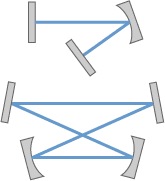
\includegraphics[scale=0.75]{linear_and_ring_resonator.png}}
\caption{Illustration of a basic optical cavity.[4]}
\end{figure}

\newpage
\section{Different Types of Optical Resonators}
\subsection{Fabry-Perot Resonator}
A system of two mirrors held parallel to each other and both having high reflectivities shows a resonant behavior at some frequencies of incident light. If both the mirrors have high reflectance, the incident light is still observed to have pass through them without any decrease in the intensity and is detected, which occurs due to phenoemnonas similar to quantum tunneling effects.

\subsection{Gires-Tournois}
It is basically a lossless Fabry-Perot resonator which have a 100$\%$ reflecting rear mirror, that means it reflects 100$\%$ at all frequencies. Still, some resonant frequencies stays between the mirrors for a longer period of time and thus descript resonant behavior and lead to ultra slow group velocities. This simple device is known for storing spectral power of light which is reflected from it while modifying its phase. That is why it is sometimes referred to as a "phase only" filter.


\section{Micro Resonators}
Microresonators are special type of resonators made from different type of materials which exhibits optical properties while being fabricated on a chip. These kind of resonators are actually useful in observing the effects of optical resonators on a device.
\subsection{Different Geometeries}
There are many type of microresonators from which microring-resonators are very useful in making photonic devices and have wide variety of application. Other kind of resonators are also useful for different kind of applications and all have distinct optical properties based on their geometery. (See figure 1.2)
\begin{figure}[h]
\centering
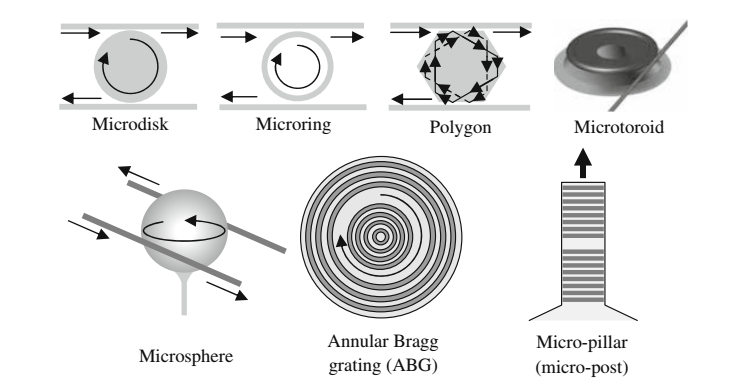
\includegraphics[width=1\textwidth]{microresonators_types.jpg}
\caption{Different geometeries of microresonators.[3]}
\end{figure}

\newpage

\section{Electromagnetically Induced Transparency and Induced Absorption (EIT and EIA)}
Electromagnetically Induced Transparency (EIT), is a coherent optical nonlinearity which makes a medium transparent to some narrow bandwidth of frequencies which were otherwise opaque to the incident radiation. This window leads to slow light at resonant frequencies in an optical resonant system usually involving coupled system. This is observed due to the destructive quantum interference effects of the incident radiation in atomic levels. [5]

\subparagraph{\normalfont \large Similarly, Electromagnetically Induced Absorption (EIA), is a similar phenomenon to EIT but in this nonlinearity the medium becomes highly opaque to some bandwidth of frequencies at resonance. Thus blocking off completely the resonant frequency radiation and causing a dip in the transmitted field. The quantum interference of light here is descructive and the atomic levels absorb the extra photons at such particular frequencies. }

\newpage
\section{Aim and Objective}
This thesis is a detailed study of such phenomenons dealing optical resonators. We will also deeply study the changing behavior of active and passive resonators. Active resonators are those resonators which are made from some gain medium and they also descript EIT and EIA like behavior in similar and distinct fashion. Then we will model the systems using different scientific tools and computation methods to predict their behavior in different circumstances and parameters. 


\newpage
\section*{References}
\addcontentsline{toc}{section}{References}

[1]  N. Uzunoglu et al., "photonics microresonator research and application," in photonics
microresonator research and appllicatin, New York, © Springer Science+Business Media,
LLC 2010, 2010, p. 515 \\ 

[2] Induced transparency and absorption in coupled whispering-gallery microresonators, PHYSICAL REVIEW A 71, 043804, published 5 April 2005

[3] https://en.wikipedia.org/wiki/Resonator \\

[4] https://www.rp-photonics.com/optical-resonators.html \\

[5] What is and what is not electromagnetically
induced transparency in whispering-gallery
microcavities, DOI: 10.1038/ncomms6082, Published 24 Oct 2014 \\